\documentclass[a4paper,10pt]{article}
\usepackage[utf8x]{inputenc}
\usepackage{hyperref}
\usepackage{epsfig}

%opening
\title{Daffodil}
\author{Alejandro Rodr\'{\i}guez}

\begin{document}

\maketitle

Daffodil is a parser generator that produces DFDL parsers from XSD schemas. It is based on the DFDL specification version 1 \href{http://forge.gridforum.org/sf/docman/do/downloadDocument/projects.dfdl-wg/docman.root.current_0/doc16037/2}{draft 42}.

A DFDL parser parses a raw document in the format described by a schema and produces a DOM tree or XML document.

\section{Requirements}

Daffodil is implemented in 100\% \href{http://www.scala-lang.org/}{Scala 2.8}.

It is not required to install Scala to run or compile Daffodil (the required Scala libraries are included in the dependencies). It does require \href{http://www.java.com/en/}{Java} 1.6 or higher.

\href{http://ant.apache.org/}{Apache Ant} (1.7 or higher) is required for building using the provided script.

All other scripts included for testing and running are Bash scripts, although Daffodil itself will run on any platform with JVM 1.6 or higher available.

\section{Dependencies}

All dependencies are included in the \$DAFFODIL/lib folder:

\begin{itemize}
 \item Scala compiler (scala-compiler.jar)
 \item Scala runtime (scala-library.jar)
 \item Scala unit testing library (scalatest-1.2.jar)
 \item Saxon-B 9.1 XPath engine (saxon9.jar, saxon9-jdom.jar, saxon9-s9api.jar, saxon9-xpath.jar, xerces.jar)
 \item JDOM (jdom.jar)
 \item Derby (derby.jar, derbytools.jar)
 \item Joda (joda-time-1.6.jar)
 \item IBM ICU 4 (icu4j-4\_4\_1\_1.jar)                           
\end{itemize}

\section{Building}

An Ant script is provided in \$DAFFODIL/build.xml.

To compile the source code and generate the daffodil.jar:

\begin{verbatim}
$ ANT_OPTS=-Xss64m; ant compile 
\end{verbatim}

To run the unit tests:

\begin{verbatim}
$ ant test
\end{verbatim}

To run the DFDL test cases:

\begin{verbatim}
$ test/runTest.sh
\end{verbatim}

\section{Running}

The provided Bash script \emph{daffodil.sh} sets the classpath and invokes Daffodil command line \emph{daffodil.Main}. 

If the Scala interpreter is installed and the classpath is already set (say in \$CLASSPATH), Daffodil can be invoked as\footnote{Daffodil uses recursion extensively and might exhaust the default stack memory limit of the JVM. \emph{daffodil.sh} sets a custom limit that should be high enough for most practical purposes.}:

\begin{verbatim}
$ scala -cp $CLASSPATH daffodil.Main [OPTIONS]
\end{verbatim}

Otherwise the easiest way to run Daffodil is through the script, as:

\begin{verbatim}
$ $DAFFODIL/daffodil.sh [OPTIONS]
\end{verbatim}


Normally Daffodil command line requires two arguments: the name of a schema file and the name of a data file. These are passed through the options:

\begin{verbatim}
$ $DAFFODIL/daffodil.sh -i <dataFile> -s <schemaFile>
\end{verbatim}


Daffodil can also store the generated DFDL parser and use it at a later time, e.g:

\begin{verbatim}
$ $DAFFODIL/daffodil.sh -s <schemaFile> -D <generatedParseFile>
$ $DAFFODIL/daffodil.sh -p <generatedParseFile> -i <schemaFile>
\end{verbatim}

The output is an XML file produced by parsing the specified data file. This output is printed to standard output unless the -o option is used. 


If the XSD schema contains more than one top level element, Daffodil must be informed of the element that should be used as root of the output XML. This can be done through the -r option.

\begin{verbatim}
$ $DAFFODIL/daffodil.sh -i <dataFile> -s <schemaFile> -r <myRootElement>
\end{verbatim}

Below is a complete list of options for the command line:

\begin{tabular}{l|p{3in}}
 -d, --debug & start the parser in interactive debugger mode. This mode helps debug the schema by printing step by step information of the parsing. \\
-D, --parser-destination $<file>$ & saves the produced parser to the specified file. \\
-g, --grddl $<grddl>$ & adds a grddl transformation (can be specified multiple times). -o needs to be specified.\\
-G,-grddlOutput $<grddl>$ & indicates the output for the grddl transformation. If not specified, $<ouput>$.rdf will be used (as specified by -o).\\
-h, --help & prints this help message. \\
-i, --input $<input>$ & the input data file to translate. \\
-o, --output $<output>$ & saves XML output to the specified file. If not specified, ouput is printed to standard output \\
-p, --parser $<file>$ & reads a previously saved parser. Use this option instead of -s if you saved the parser.\\
-r, --root $<root>$ & the root element of the XML file to produce. This needs to be one of the top-level elements of the DFDL schema.\\
-s, --schema $<schema>$ & the annotated DFDL schema to use to produce the parser.\\
-v, --version &  prints version information and exits. \\
-V, --verbose &  prints additional information while processing and on errors. \\
\end{tabular}

\section{Folder Structure}

\begin{description}
 \item [\$DAFFODIL/src] The scala source code (excluding unit testing).
 \item [\$DAFFODIL/updatedSrcTest] The scala source code for unit testing.
 \item [\$DAFFODIL/test] DFDL test cases. This folder includes DFDL schemas (*.xsd), with corresponding input files (*.in) and expected output (*.xml). Two scripts, \emph{runTest.sh} and \emph{serializationTest.sh}, automatically run the whole test suite. \emph{runTest.sh} directly generates the output for each test case from the schema and the input while \emph{serializationTest.sh} tests the additional step of saving the generated parser to a file, then loading it and using it to generate the output. The file \emph{testSuite.txt} lists the test cases used by the scripts.
 \item [\$DAFFODIL/lib] The dependency jars.
 \item [\$DAFFODIL/bin] The compiled binaries and the daffodil.jar with all the compiled classes.
 \item [\$DAFFODIL/doc] Documentation files.
\item [\$DAFFODIL/.idea] IntelliJ Idea project files.

\end{description}

\section{Development Environment}

Daffodil is not dependent on any particular IDE. However, most development was done in IntelliJ Idea and a project file is included (\$DAFFODIL/.idea).
Idea requires a Scala plugin, available in the default installation but not enable by default (Enable through $File -> Settings -> Plugins -> Available$).
Also, as of September 2010, Idea scala plugin only includes the libraries for scala 2.7. Scala 2.8 libraries need to be manually installed in
\$HOME/.Idea<VERSION>/config/plugins/Scala.


Daffodil VCS of choice is Baazar.

\section{Architecture}

\begin{figure}[htp]
\hspace{-1.5cm}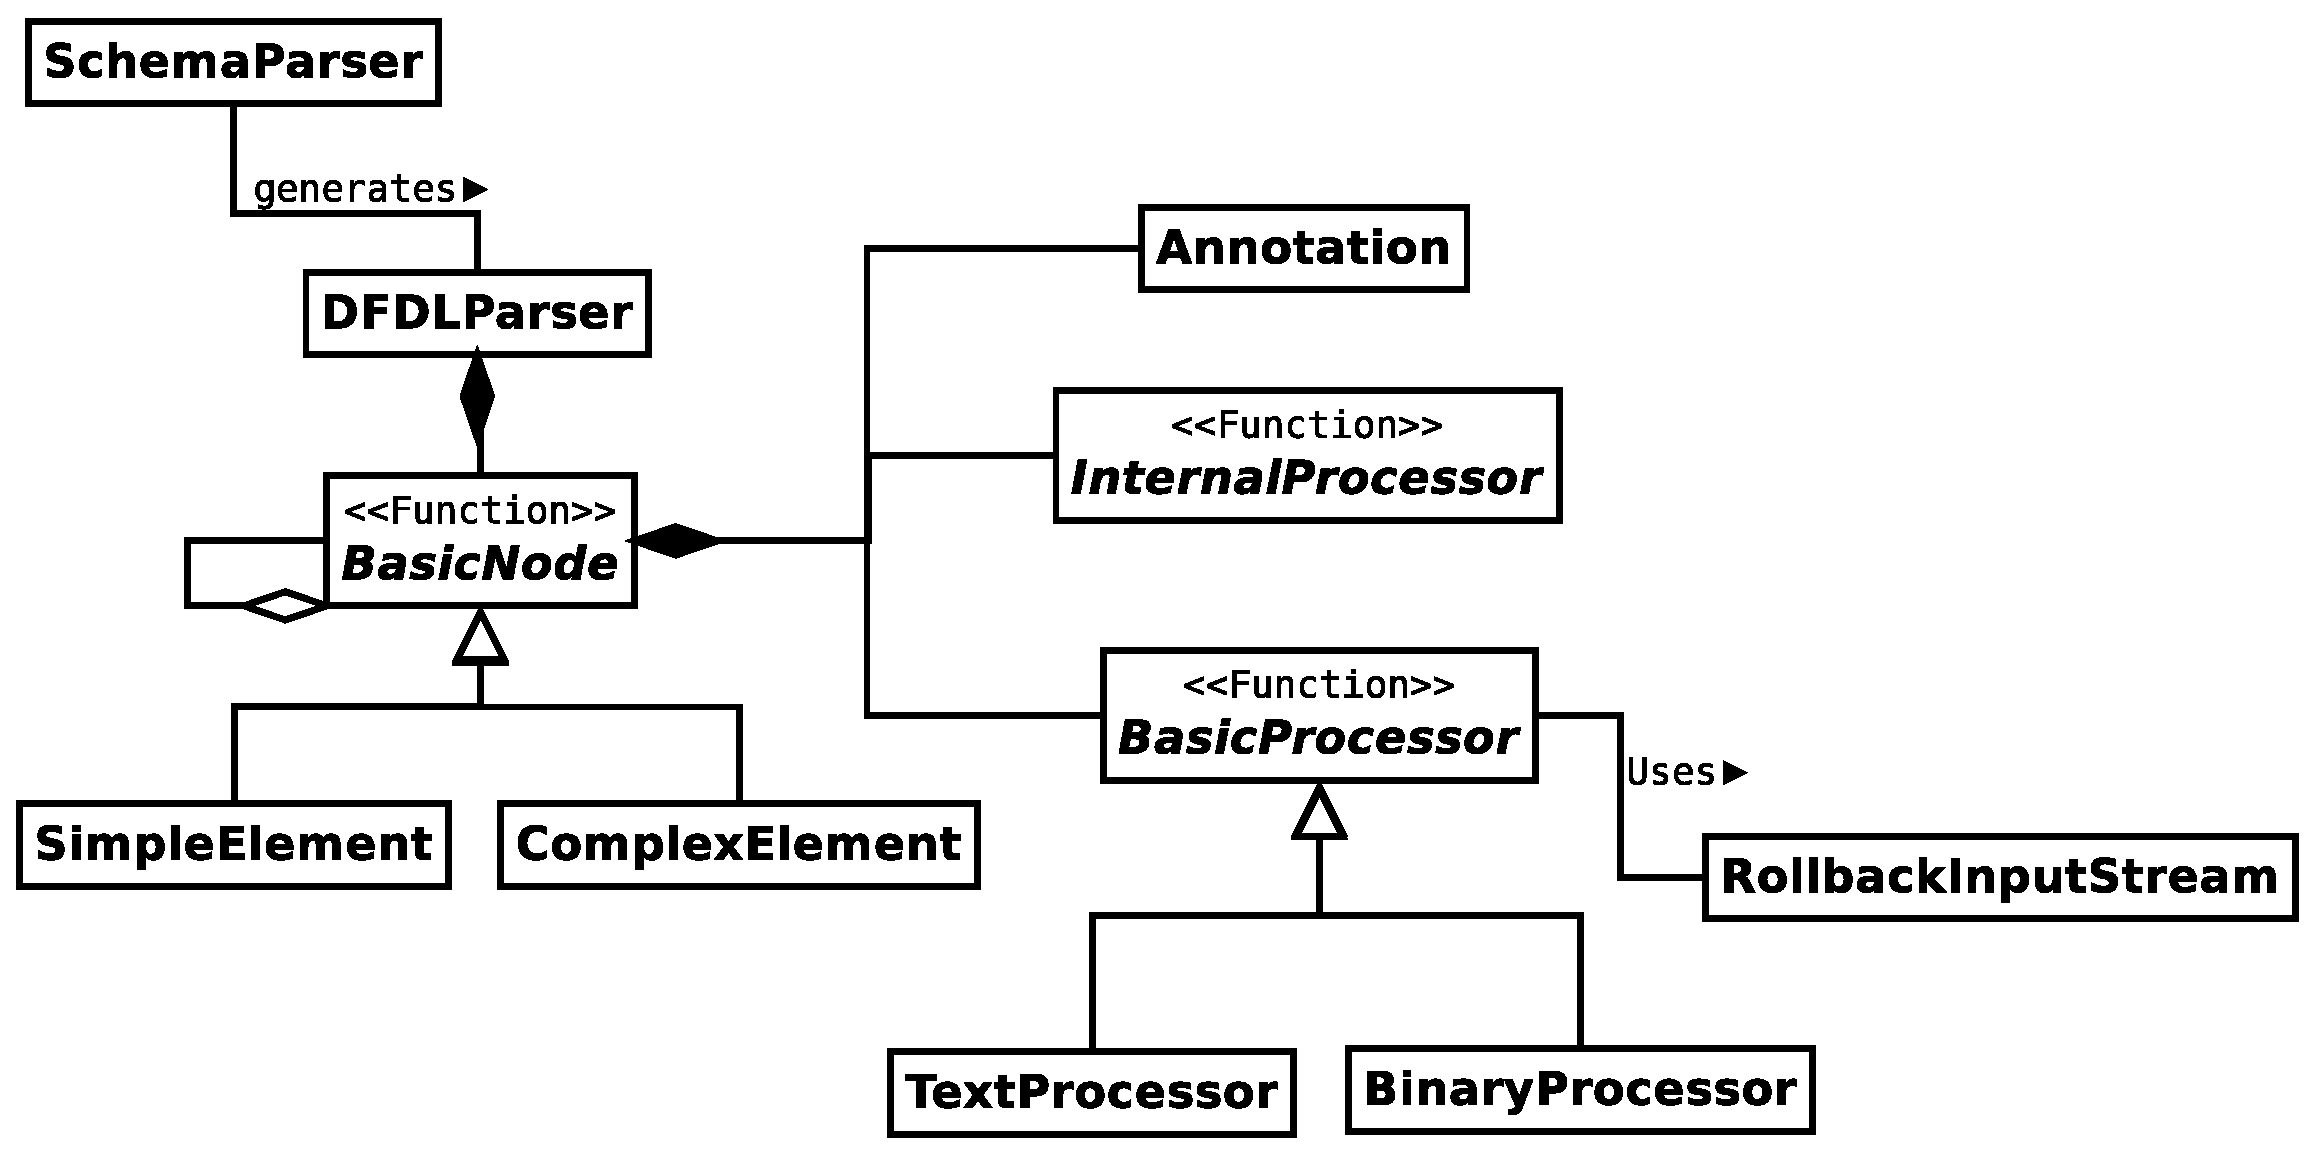
\epsfig{file=structure.eps,width=15cm}
%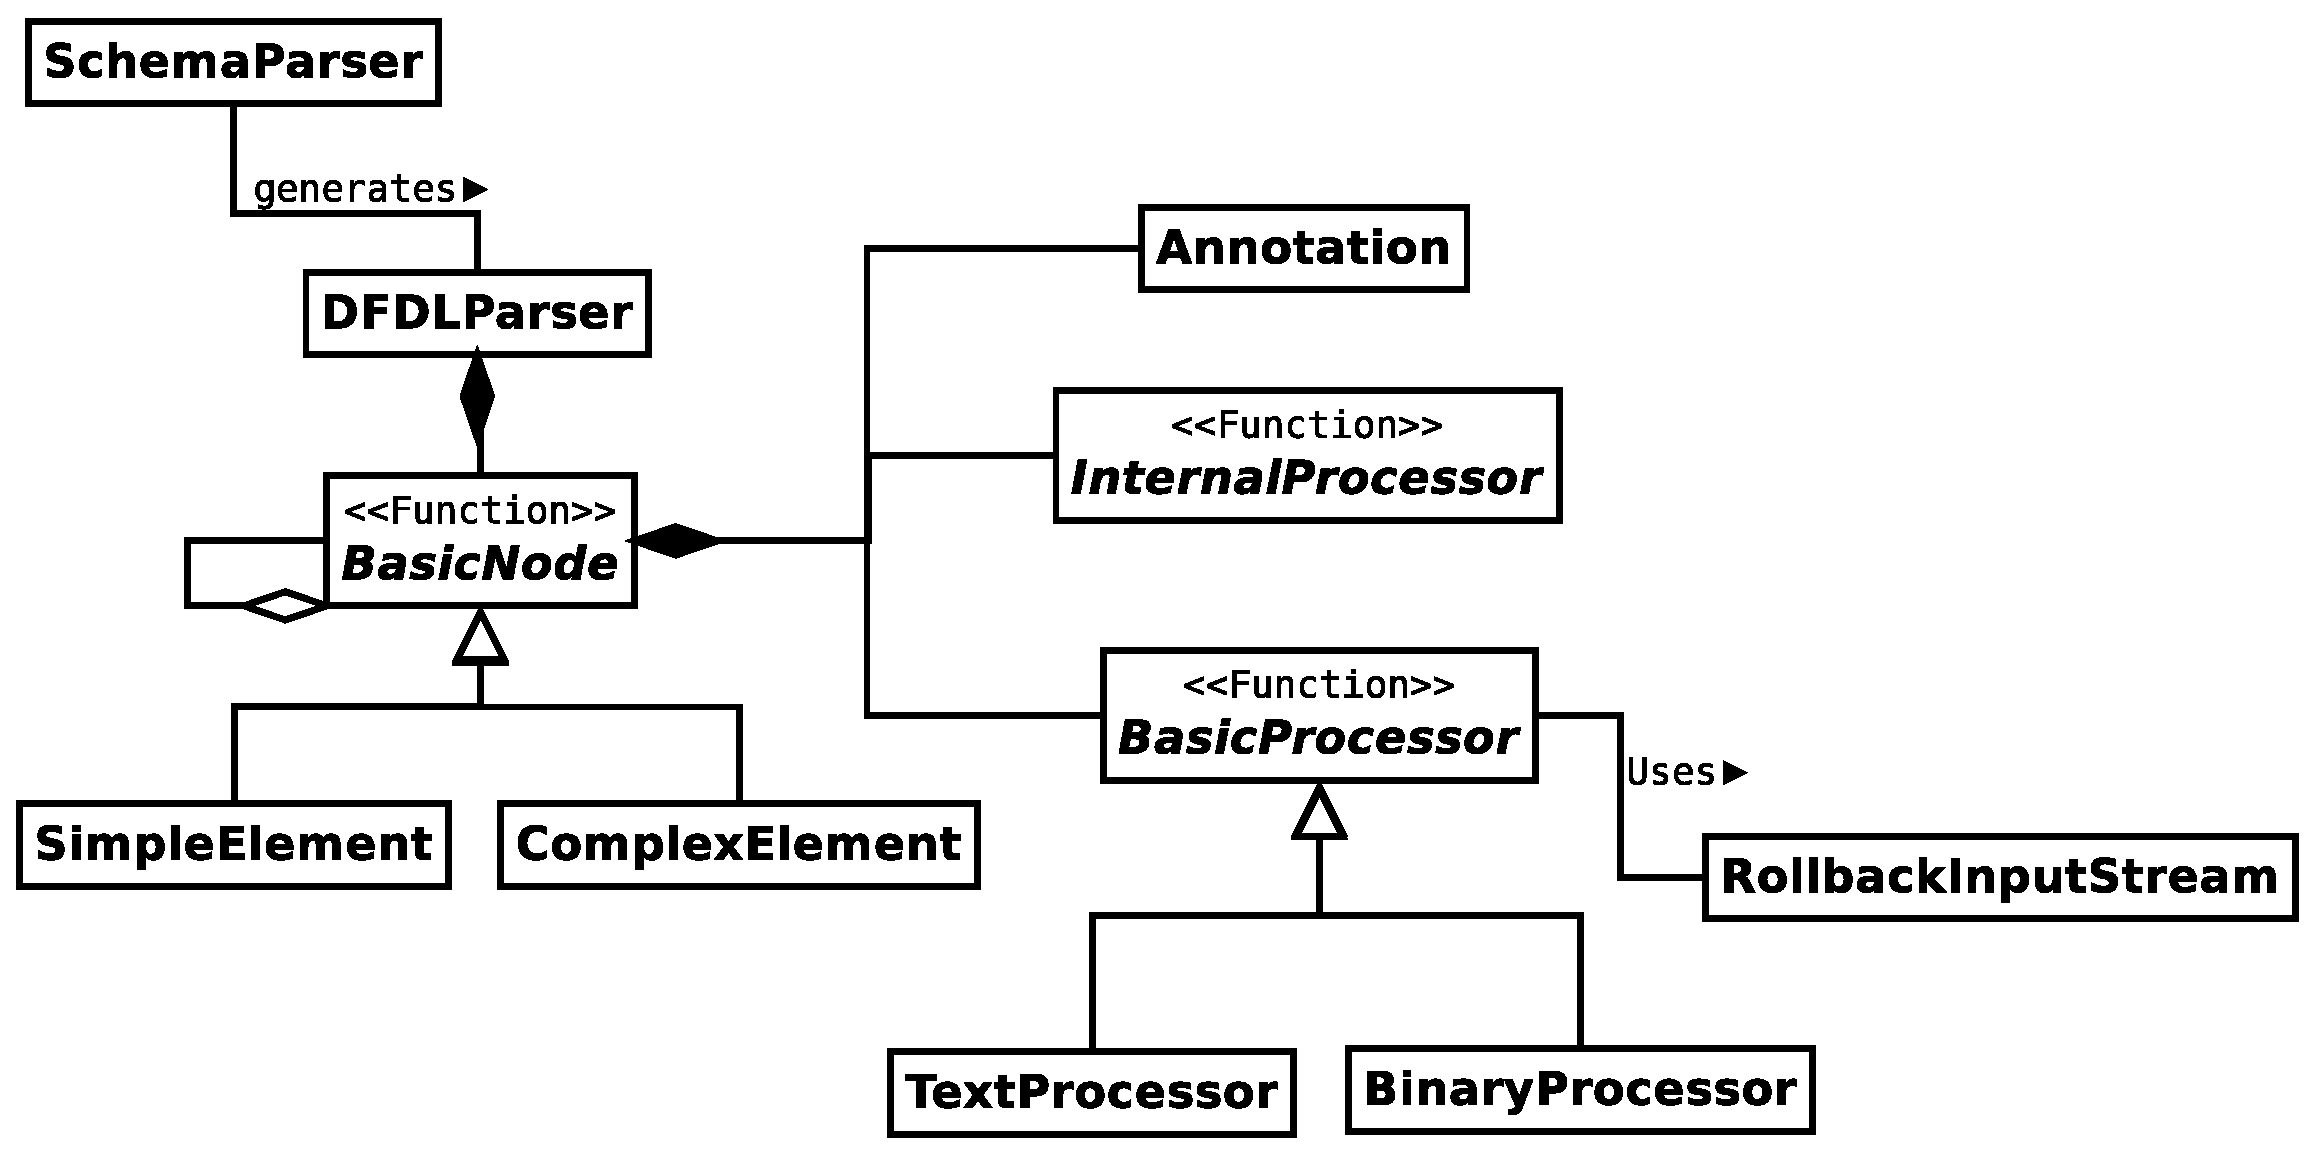
\includegraphics{./structure}[height=5cm]
 % structure.eps: 0x0 pixel, 300dpi, 0.00x0.00 cm, bb=0 0 1134 538
\caption{Simplified Structure}
\end{figure}

\subsection{Basic Description}
Daffodil takes a DFDL schema and produces a forest of logical parsers (collection of trees of BasicNodes), where each logical parser corresponds more or less to each component described in the DFDL schema. A logical parser (BasicNode) is a function that takes an input stream (which current position should reflect the bytes that correspond to the logical DOM element) and a context node in a DOM tree (the parent node of the XML element to be parsed) and produces the associated logical element by parsing the input and delegating to children logical parsers as needed.

Since DFDL possibly needs to evaluate XPath expressions on backward references, the tree is not built bottom-up, so a BasicNode actually adds DOM nodes to the context node before delegating to children nodes. In the case of a processing error (an error that a DFDL parser should backtrack, signaled by an ElementProcessingException), the BasicNode should cause no side effects on its arguments.

Actual reading of the input stream, including scanning of text, transformation of binary values into text values, etc., is delegated to processors (BasicProcessor and InternalProcessor), that are responsible for understanding the physical format associated to a logical element.
 
\subsection{Description of Main Clases}

\subsubsection{SchemaParser}

SchemaParser takes a DFDL schema and produces a DFDLParser. SchemaParser and its component AnnotationParser are responsible for understanding an XSD Schema and all the DFDL annotations and mapping them into a DFDLParser.

\subsubsection{DFDLParser}

A DFDLParser is an immutable object that holds a collection of BasicNodes, one for each top-level element, group  and type defined in the DFDL schema, and acts as the initial dispatcher in the parsing process by invoking the BasicNode corresponding to the root of the output DOM tree.

\subsubsection{BasicNode}

A BasicNode is a function corresponding to a logical component of the schema. A logical component might be an element, complex type, group, etc. A BasicNode takes the input stream and produces the corresponding DOM element resulting from parsing the input stream at its current position. If an element might occur multiple consecutive times, BasicNode will generate all the consecutive occurrences and add them to the DOM tree.

Each BasicNode holds an Annotation object with all the information about the physical format of the node, plus information about minimum and maximum number of occurrences, xsd:type, etc.

BasicNodes are immutable and should have no memory of previous invocations.

\subsubsection{SimpleElement}

A BasicNode corresponding to the xsd:simpleElement component. SimpleElements have no children nodes.

\subsubsection{ComplexElement}

A BasicNode corresponding to the xsd:complextElement component. A ComplexElement nests an xsd:sequence or xsd:choice node.

\subsubsection{Annotation}

A data structure to hold all the information about the physical format of a node, plus additional properties of a logical element, such as xsd:type, number of occurrences, etc. Annotations can nest other annotations.

\subsubsection{BasicProcessor}

BasicProcessors are functions that perform the physical reading from the raw input and return a text value corresponding to the text value of the logical element parsed. As functions/objects, they actually have three possible invocations: init (scan initiators, consume padding, align to proper byte, etc.), apply (gets text value of next element) and terminate (consume terminators, consume padding). BasicProcessors also perform the required conversions from the values read from the input to the appropriate value for the xsd:type of the element.

BasicProcessors are immutable and should have no memory of previous invocations.

\subsubsection{InternalProcessor}

InternalProcessors are functions that represent actions that do not consume input nor produce outputs. These are actions are perform before or after processing an element, such as evaluating assertions, binding DFDL variables, etc.

InternalProcessors are immutable and should have no memory of previous invocations.

\subsubsection{RollbackInputStream}

An input stream that allows stackable marks, that is, maintains a stack of checkpoints to return the stream to a previous state.

\subsubsection{Main}

Provides command line access to SchemaParser and DFDLParser classes.

\section{Known Issues}

\begin{itemize}
 \item Daffodil keeps a fixed-size buffer of the input stream to avoid putting the whole input file in memory. Pushing back further than the size of the buffer will cause an exception.
 \item RollbackInputStream reads an input stream one byte at a time and maintains alignment to byte. DFDL specification allows alignment to bits.
 \item SchemaParser does not resolve external references (references to elements or types in schemas other than the one passed to SchemaParser).
 \item SchemaParser and DFDLParser and condensed into one.
\end{itemize}

\end{document}
